\documentclass[a4paper, 1.5lines]{ctexart}
\usepackage[top=3cm, bottom=2cm]{geometry}
\usepackage{graphicx}
\usepackage{subcaption}
\usepackage{amsmath}
\usepackage{xcolor}
\usepackage{url}
\usepackage{booktabs}
\usepackage{multirow}
%\usepackage{hyperref}
\usepackage[hidelinks]{hyperref} % 加载 hyperref 并隐藏链接边框

%\usepackage[utf8]{inputenc}
%\usepackage[ngerman]{babel} % 加载德语支持

% booktabs 提供 \toprule, \midrule, \bottomrule 等表格命令
\usepackage{booktabs}
% 定义占位命令以避免未定义控制序列错误
\newcommand{\placeholderspace}{}
\usepackage{fancyhdr} % 导入fancyhdr宏包
\usepackage{lipsum}   % 仅用于生成示例文本
\usepackage{float}    % 提供 H 浮动位置选项

% 设置页面样式为fancy
\pagestyle{fancy}
% 自定义页眉内容
\fancyhead[L]{} % 左侧页眉
\fancyhead[C]{\textbf{Physics-experiment Reporting Letter:\\Optical Multi-channel and H-D spectroscopy}} % 中间页眉
\fancyhead[R]{ } % 右侧页眉
% 自定义页脚内容
\fancyfoot[L]{ } % 左侧页脚
\fancyfoot[C]{\thepage} % 中间页脚显示页码
\fancyfoot[R]{ } % 右侧页脚
% 改变页眉线的粗细
\renewcommand{\headrulewidth}{1.4pt}
% 改变页脚线的粗细
\renewcommand{\footrulewidth}{0.pt}





\title{光学多道与氢氘同位素光谱}
\author{实验人：唐亿\qquad 学号：202311998381\qquad 指导教师：弓文平}
\date{实验日期：2025.11.7}


\begin{document}
    
    \maketitle
    
    \begin{abstract}
         光谱学技术在许多领域中都具有重要价值。本实验借助光学多道分析仪对氢原子及其同位素的光谱进行了研究，测得了氢、氘在可见光区域的谱线波长，并据此计算了对应的Rydberg常数。同时，利用同位素位移所包含的光学信息求得了电子与质子的质量比。文章还对实验中可能产生的误差来源进行了分析，并探讨了进一步提升测量精度的可能途径。

         \textbf{\textbf{关键词：氢氘光谱\quad CCD\quad PMT\quad Rydberg常数}}
    \end{abstract}
    
    \section{引言}
       光谱学在物理学的多个分支中具有核心地位，包括原子与分子物理、天体物理、等离子体物理、激光物理以及材料物理等。同时，它在计量、化学、生物、医学、刑侦、地质、冶金、矿物及考古等领域也发挥着重要作用，被广泛用于分析材料结构参数、诊断物质的物理性质，以及进行元素的定性与定量检测。

本实验利用光学多道分析仪对氢原子同位素的光谱特性进行研究，并分别采用 CCD 与 PMT 测量氢与氘在可见光区域的谱线。通过这些测量，可以比较 H 与 D 原子谱线的差异，同时熟悉光学多道分析仪的工作方式与常用的光谱测量技术。

    \section{原理}
        \subsection{Bohr的原子模型}
       原子在能级之间跃迁时会伴随光子的吸收或放出，其频率满足关系式 $\nu = \Delta E / h$。由于原子能级是离散的，能量只能取特定的量子值，因此原子只能与某些特定频率的光发生作用。这些特定频率的辐射在分光仪上呈现为离散的谱线，即所谓的原子光谱。对于原子光谱的最初经验性描述源于Balmer公式，其形式为：
            
        \centerline{$\dfrac{1}{\lambda} = R \left(\dfrac{1}{n_1^2} - \dfrac{1}{n_2^2}\right)$}

        其中$\lambda$为光的波长，$n_1$、$n_2$为能级数，$R$为Rydberg常数。

        不同原子的Rydberg常数一般不同。根据Bohr的半经典模型，有

        \centerline{$R = R_{\infty}\dfrac{m_n}{m_n + m_e}$}

        其中$ m_n $为原子核质量，$m_e $为电子质量。

        对于氢 H 与氘 D 这两种同位素，它们都只有一个核外电子，但氘核由一个质子和一个中子组成，而氢核仅含一个质子。忽略中子和质子静止质量的差异，可得
        \begin{align*}
            R_H &= R_{\infty}\frac{m_p}{m_p + m_e}\\
            R_D &= R_{\infty}\frac{2m_p}{2m_p + m_e}
        \end{align*}

        因此，同类型跃迁对应的谱线波长差满足

        \centerline{$\Delta\lambda= \dfrac{1}{R_{\infty}}\dfrac{m_e}{2m_p}\left(\dfrac{1}{n_1^2}-\dfrac{1}{n_2^2}\right)^{-1}= \dfrac{m_e}{2m_p + m_e}\lambda_D$}

        其中$ \Delta\lambda $表示氢与氘的谱线波长之差。该结果说明二者的谱线位置并不完全相同，从而产生同位素位移。

        进一步可得近似关系

        \centerline{$\dfrac{\Delta\lambda}{\lambda_D} \approx \dfrac{m_e}{2m_p}$}

        这一路径使得可通过光谱测量估算电子与质子的质量比。

        \subsection{氢、氘谱线的真空波长理论值}
        根据Balmer公式，取氢的Rydberg常数$ R_H = 109677.58\ \mathrm{cm^{-1}}$ 与氘的Rydberg常数 $R_D = 109707.42\ \mathrm{cm^{-1}}$，计算元素从能级 $n=3,4,5,6$ 跃迁到 $n=2$ 的四条谱线在真空中的理论波长，计算结果列于表\ref{tab:theory_wavelength}中。

        \begin{table}[h]
            \centering
            \caption{氢、氘谱线在真空中的理论波长}
            \label{tab:hd-wavelengths}
            \begin{tabular}{@{} c c c c c @{}}
            \toprule
            $n$ & $3$ & $4$ & $5$ & $6$ \\
            \midrule
            $\lambda_{H}\ /\ \mathrm{nm}$ & 656.47 & 486.27 & 434.17 & 410.29 \\
            $\lambda_{D}\ /\ \mathrm{nm}$ & 656.29 & 486.14 & 434.05 & 410.18 \\
            $\Delta\lambda\ /\ \mathrm{nm}$ & 0.18 & 0.13 & 0.12 & 0.11 \\
            \bottomrule
            \end{tabular}
            \label{tab:theory_wavelength}
        \end{table}

        \subsection{真空修正}
        实验中得到的谱线波长对应的是空气条件下的数值。为了将其换算为真空中的波长，需要利用折射率修正关系式:

        \centerline{$n - 1 = \dfrac{n_g - 1}{1 + at} \dfrac{P}{P_0} - \dfrac{be}{1 + at}$}
        
        \centerline{$n_g = 1 + A + \dfrac{3}{\lambda^2}B + \dfrac{5}{\lambda^4}C$}

        式中 $t$ 为室温，$P$ 为实验室气压，$e$ 表示水蒸气压，$n_g$ 为标准状况下的群折射率，而 $n$ 则为空气在实验条件下的折射率。在常规实验条件下，折射率的气压项与湿度项的影响通常较小，因此只需采用上面的形式对折射率进行校正即可。
    
        给定空气中所测得的波长$ \lambda$，其对应的真空波长可表示为

        \centerline{$\lambda_0 = n_g \lambda$}

        \subsection{实验分光原理}
        本实验所使用的光学多色仪采用平面反射式光栅作为色散元件，其满足光栅方程

        \centerline{$a(\sin\gamma + \sin\beta) = m\lambda$},

        其中 $m$ 为衍射级次，$a$ 为光栅常数，$\gamma$ 与 $\beta$ 分别表示入射光与出射光相对于光栅法线的夹角。该关系式说明不同波长的光对应着不同的出射角度，从而实现了光的空间分离。

        光栅光谱仪的角色散率可写为

        \centerline{$\dfrac{\mathrm{d}\theta}{\mathrm{d}\lambda} = \dfrac{m}{a\cos\theta}$}

        在衍射角$ \theta \ll 1 $的情况下，$\cos\theta $近似为常数，因此出射方向与波长之间的关系可以视为线性，这使得探测器上的空间位置与波长一一对应。

        光栅光谱仪的分辨本领由

        \centerline{$R = mN$}

        给出，其中 N 为光栅上的总刻线数。对光栅常数相同的光栅而言，刻划面的尺寸越大，对应的刻线总数越多，其可达分辨本领也越高。然而在实际实验中，入射光束通常无法完全照射整个刻划面，因此只有被光束照亮的刻线区域才真正对分辨本领起作用。

    \section{实验}
        \subsection{实验内容}
        本实验借助光学多道分析仪对氢与氘的发射光谱进行测量，从而获得两者谱线位置及其同位素位移。在此基础上计算里德堡常数与电子—质子质量比，并进一步绘制氢原子的能级结构图。
        
        实验的数据采集依赖光信号向电信号的转换，而这一转换通常通过电荷耦合器件（CCD）或光电倍增管（PMT）完成。采用 CCD 进行测量时，需要利用 He 灯或 Ne 灯的已知谱线对仪器进行波长定标；若使用 PMT，则需借助 CCD 的定标结果来修正系统的零点偏移，使测量数据能够准确反映实际波长。

        \subsection{实验仪器}
            \subsubsection{光学多色仪}
            光谱仪是一种用于将复色光分离为光谱的光学仪器，主要由准直系统、色散系统和成像系统三部分构成。当在像平面处安装出射狭缝时，经色散系统分离后的单色光可以依次从狭缝出射，此类仪器称为单色仪；若像平面处布置一系列狭缝或矩形开口，使多个单色光能够同时出射，则称为多色仪。单色仪或多色仪的狭缝后通常配有光电转换元件，用于记录光谱信息。

            入射光依次经反射镜 $\mathrm{M}_1$ 和准光镜 $\mathrm{M}_2$ 反射后照射到光栅上，光栅的衍射作用使不同波长的光沿不同方向传播。衍射光再经与 $\mathrm{M}_1$ 和 $\mathrm{M}_2$ 对称布置的平面镜 $\mathrm{M}_3$ 和 $\mathrm{M}_4$ 反射后进入 CCD 光电探测器或光电倍增管，实现光谱信号的接收与记录。

            结构如图\ref{fig:yiqi}所示。
            \begin{figure}
                \centering
                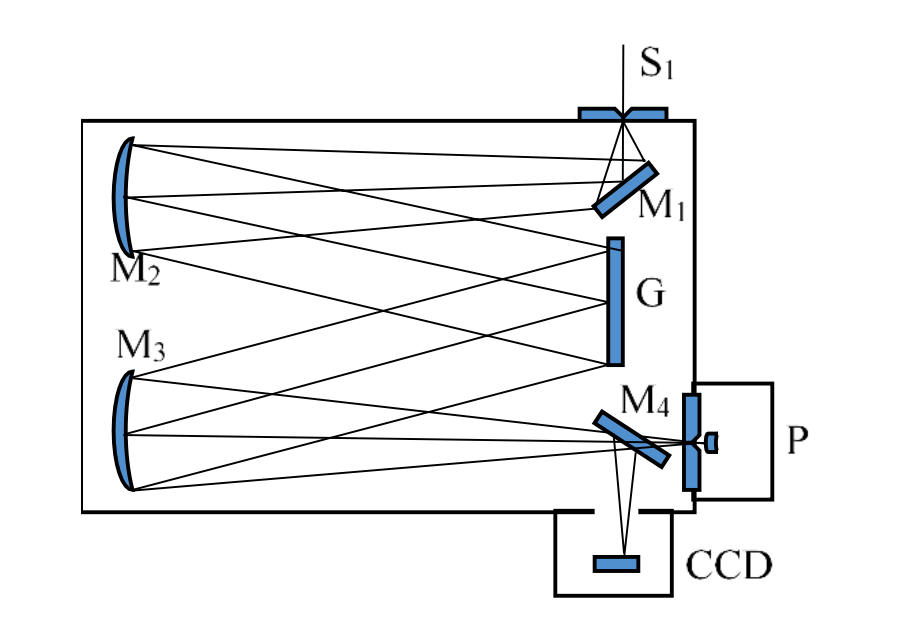
\includegraphics[width=100mm]{fig//仪器.png}
                \caption{光学多色仪示意图}
                \label{fig:yiqi}
            \end{figure}

            \subsubsection{CCD}
            CCD 探测器件由金属氧化物半导体制成的光电转换二极管作为感光像元，这些像元以面阵列或线阵列方式排列形成固体成像器件。光电转换二极管能够将入射光子转换为信号电荷，并完成电荷的存储、转移与读出。当二极管受到光照时，被吸收的光子产生电子–空穴对，其中电子被吸引至电荷反型区，实现电荷的存储。通过向 CCD 各像元的电极施加按一定规律变化的电压脉冲，电极下形成的电荷包便可沿半导体表面按设定方向移动，从而实现电荷的逐级转移。最终，转移至 CCD 输出端的信号电荷在输出电路中通过电荷–电压（或电流）的线性变换被读出，完成光信号向电信号的转换。

            \subsubsection{PMT}
            光电倍增管是一种能够将微弱光信号转化为电信号的真空电子器件，具有极高的探测灵敏度和极快的时间响应，可用于紫外、可见以及近红外波段的光信号探测。它通常由光电发射阴极（光阴极）、聚焦电极、电子倍增极以及电子收集极（阳极）等部分构成。当光照射到光阴极时，光阴极会向真空中发射光电子。这些光电子在聚焦电极形成的电场作用下进入倍增系统，并通过连续的二次发射过程得到逐级放大。随后，放大的电子束被阳极收集并输出为电信号。在实际应用中，光电倍增管的工作电压对光信号的探测性能具有重要影响：提高工作电压能够增强信号增益，但若电压过高，则可能造成信号失真，甚至引发光电极损坏。

        \subsection{实验定标}
        由于 CCD 和 PMT 只能精确记录光谱中心波长附近各位置波长的相对关系，且随着仪器长期使用，其内部元件的位置可能发生微小偏移，因此必须借助标准光谱进行波长定标。在 CCD 测量中，选用 He 灯（用于 $n=4,5,6$ 能级跃迁）和 Ne 灯（用于 $n=3$ 能级跃迁）作为定标光源。随后，利用测得的氢光谱谱线对 PMT 测量氢氘混合光源进行定标，以消除仪器零点偏差并保证测量精度。
    \section{结果与分析讨论}
        考虑到实验室所提供的 CCD 和 PMT 仪器特点，本实验采用 CCD 测量氢原子光谱谱线波长，而利用 PMT 测量氘原子光谱谱线波长。在氢光谱测量中，使用了 H 灯、He 灯和 Ne 灯作为光源，并借助 He 灯与 Ne 灯的已知谱线进行波长定标，从而测得 $\mathrm{H}_{\alpha}$、$\mathrm{H}_{\beta}$、$\mathrm{H}_{\gamma}$ 以及 $\mathrm{H}_{\delta}$ 四条谱线的波长。在氘光谱测量中，使用 H–D 混合气体灯作为光源，并利用 CCD 测得的氢谱线数据进行定标，测定了 $\mathrm{D}_{\alpha}$、$\mathrm{D}_{\beta}$、$\mathrm{D}_{\gamma}$ 和 $\mathrm{D}_{\delta}$ 四条谱线的波长，同时计算了氢、氘谱线的波长差。
        
        \subsection{CCD测量}
        
            \subsubsection{$n=3$谱线}
    \begin{figure}[h!]
        \centering
        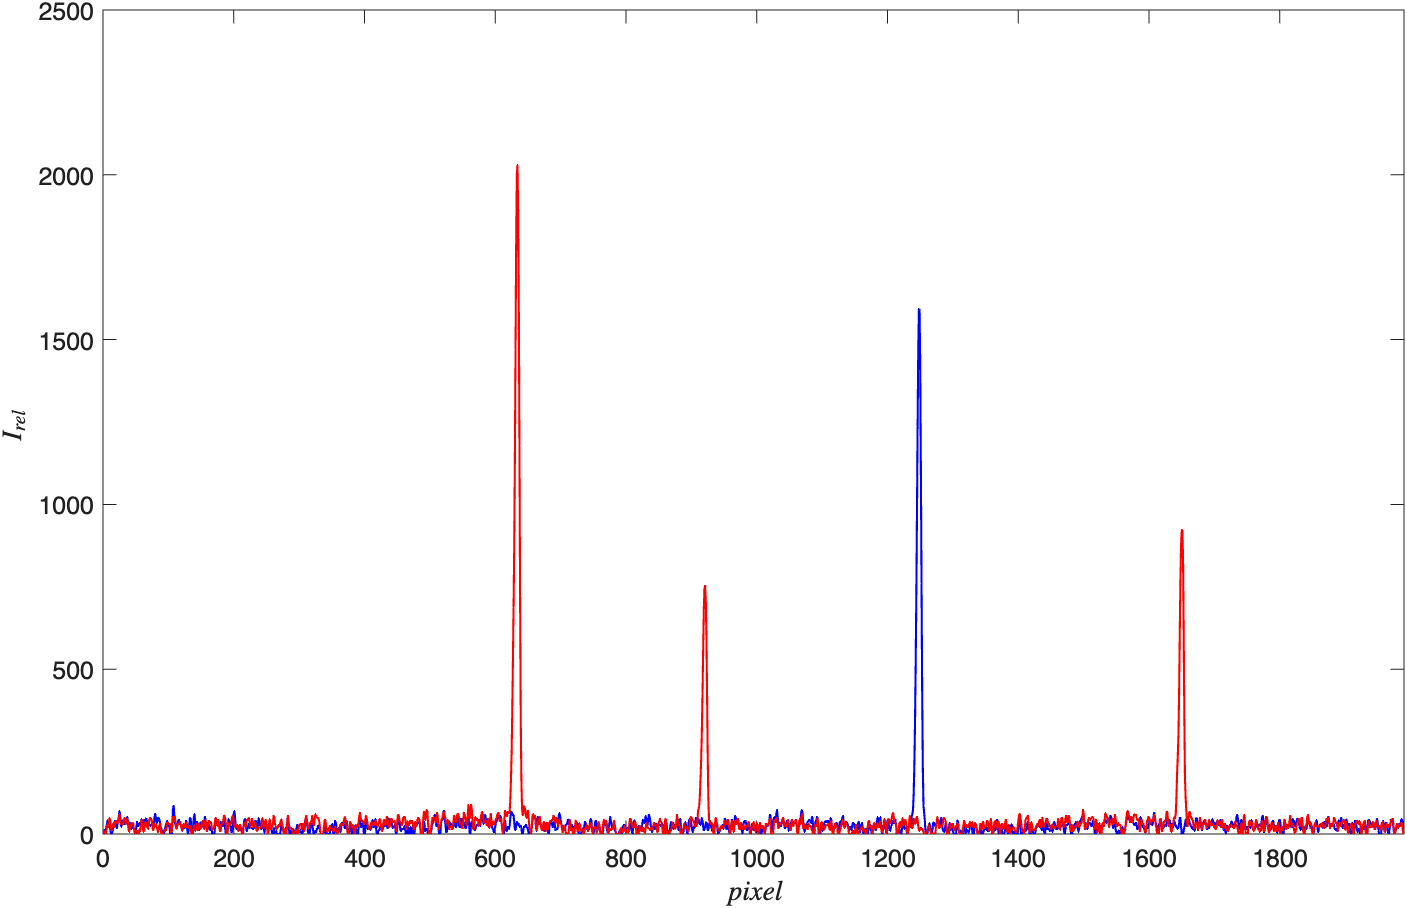
\includegraphics[width=\textwidth]{fig//h3.png}
        \caption{使用CCD测得的$\mathrm{H}_\alpha$谱线}
        \label{fig:h3}
    \end{figure}
            下面我们以$\mathrm{H}_\alpha$为例，简述一下定标的具体细节：

            我们可以通过软件寻峰得到三个Ne的像素坐标值，分别记为$px_1,px_2,px_3$。同时，我们知道理论上他们的波长为$\lambda_1,\lambda_2,\lambda_3$。
            我们采用线性定标，利用第一条和第二条来定标。则我们能得到拟合的第三条波长

            \centerline{$\bar{\lambda}_3 = \lambda_1 + \dfrac{px_3 - px_1}{px_2-px_1}(\lambda_2 - \lambda_1)$}

            如果满足$\bar{\lambda}_3 - \lambda_3 \le 0.05\mathrm{nm}$，则说明线性程度良好，我们用其得到H的波长。

            \centerline{$\bar{\lambda}_H = \lambda_1 + \dfrac{px_H - px_1}{px_2-px_1}(\lambda_2 - \lambda_1)$}

            使用 Ne 灯的  $\lambda_1 = 650.65$nm 和 $\lambda_2 = 659.90$nm 两条谱线定标，测得中间谱线的波长为$\lambda_3 = 653.263$nm，与标准值$\lambda = 653.29$nm相比误差小于$0.05$nm，表明定标成功。以此测得$\mathrm{H}_{\alpha}$线的波长$\lambda_{H} = 656.222$nm
            \subsubsection{$n=4$谱线}
            使用 He 灯的 $\lambda_1 = 492.19$nm 和 $\lambda_2 = 504.77$nm 两条谱线定标,测得中间谱线的波长为$\lambda_3 = 501.547$nm，与标准值$\lambda = 501.57$nm 相比误差小于$0.05$nm，表明定标成功。以此测得$\mathrm{H}_{\beta}$线的波长$\lambda_{H} = 486.356$nm
            \subsubsection{$n=5$谱线}
            使用 He 灯的 $\lambda_1 = 438.79$nm 和 $\lambda_2 = 447.15$nm 两条谱线定标,测得中间谱线的波长为$\lambda_3 = 443.737$nm ，与标准值$\lambda = 443.74$nm 相比误差小于$0.05$nm，表明定标成功。以此测得$\mathrm{H}_{\gamma}$线的波长$\lambda_{H} = 434.127$nm
            \subsubsection{$n=6$谱线}
        \begin{figure}[h!]
            \centering
            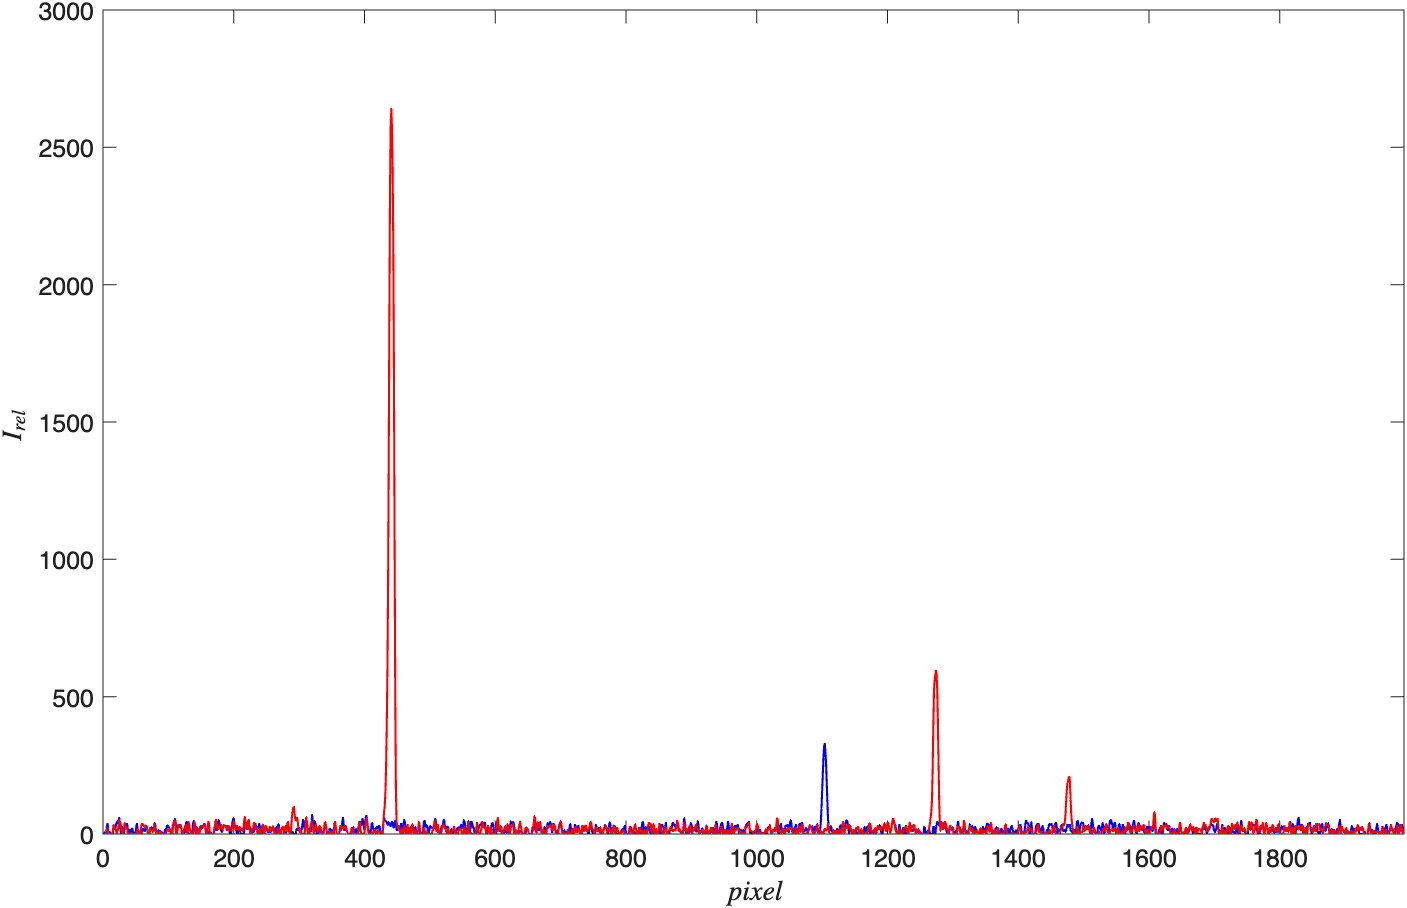
\includegraphics[width=\textwidth]{fig//h6.png}
            \caption{使用CCD测得的$\mathrm{H}_\delta$谱线}
        \label{fig:h6}
        \end{figure}
            使用 He 灯的 $\lambda_1 = 402.62$nm 和 $\lambda_2 = 414.38$nm 两条谱线定标,测得中间谱线的波长为$\lambda_3 = 412.076$nm ，与标准值$\lambda = 414.08$nm 相比误差小于$0.05$nm，表明定标成功。以此测得$\mathrm{H}_{\delta}$线的波长$\lambda_{H} = 410.146$nm

        \subsection{PMT测量}
        使用 PMT 对 H、D 灯在 400 至 660 nm 波段的光谱进行扫描，如\ref{fig:hd}所示，可以清楚地观察到若干明显的特征谱线。在此基础上，对每条谱线所在的局部波段进行更精细的扫描，并利用软件的自动寻峰功能测定 H 与 D 谱线的波长。
        \begin{figure}[h!]
            \centering
            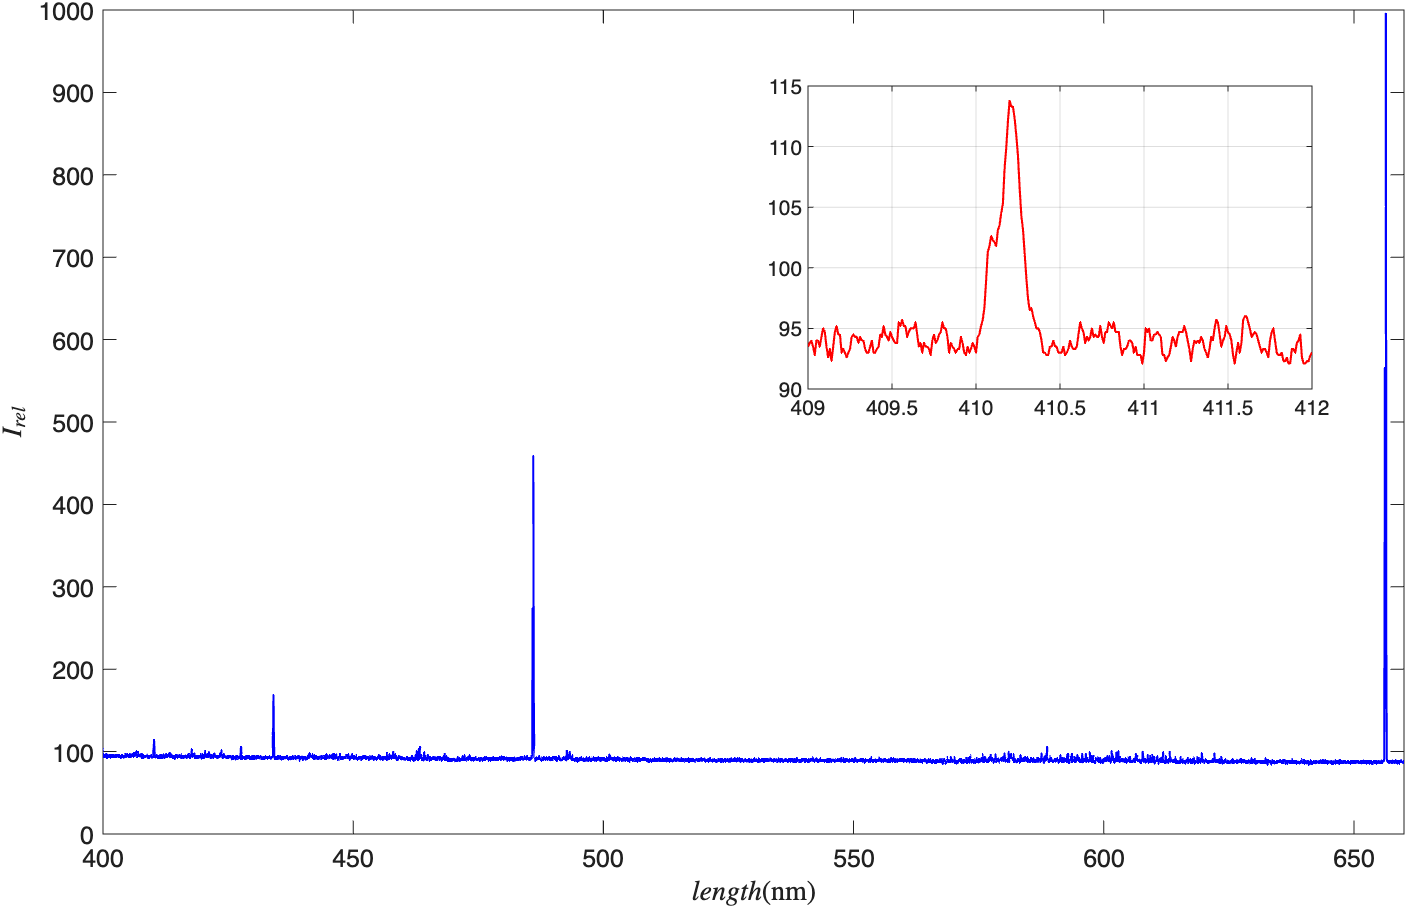
\includegraphics[width=\textwidth]{fig//hd.png}
            \caption{使用PMT测得的氢氘谱线}
        \label{fig:hd}
        \end{figure}

        \subsection{Rydberg常数}
    
        考虑到实验数据有限，Rydberg常数的测量值可由 $n$ 依次取3、4、5、6 的计算结果取平均得到，$R_H = 109663.54\mathrm{cm}^{-1},R_D = 109694.01\mathrm{cm}^{-1}$。
        \subsection{H的能级图}
    
    计算各谱线所对应的光谱项$\bar{R}_H/n^2$，以光谱项的负值为纵坐标，以$n\to\infty$时的光谱项的值为原点，用横线表示氢原子的能级画出氢的能级图，如图\ref{fig:H_energy_level}所示。
    
    \begin{figure}[h!]
        \centering
        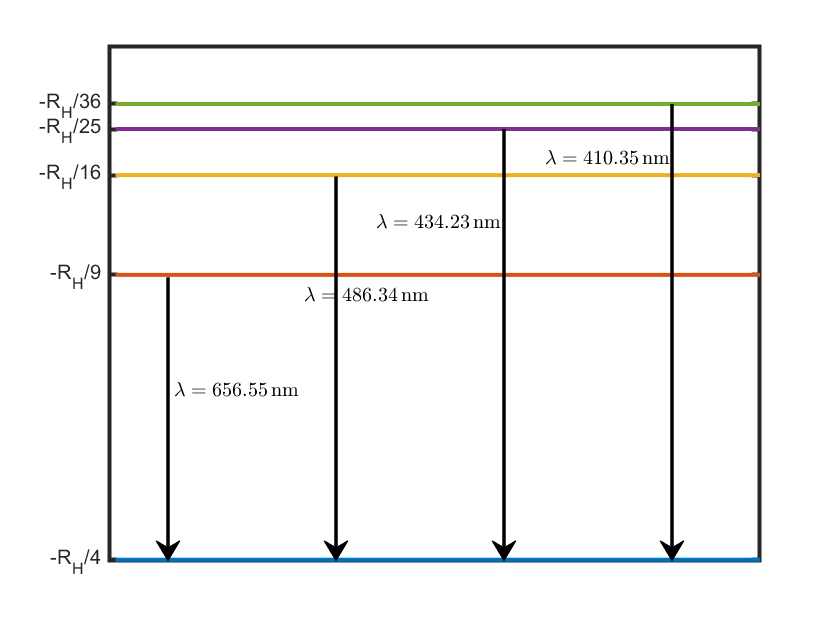
\includegraphics[width=\textwidth]{fig//energy_trans}
        \caption{H的能级图}
        \label{fig:H_energy_level}
    \end{figure}

    \subsection{电子与质子的质量比}
    
    根据公式计算的结果如表\ref{data:000}所示。电子质子质量比的最终计算结果为 $$ \dfrac{m_e}{m_p} \approx  5.557\times 10^{-4} $$
    
    该比值的标准值为
    $$ \dfrac{m_e}{m_p} \approx \dfrac{1}{1836.5} =  5.445 \times 10^{-4} $$
    
    \begin{table}[h!]
        \centering
        \caption{里德堡常数和电子质子质量比的计算结果}
        \label{data:000}
        
        \begin{tabular}{|c|c|c|c|c|c|}
            \hline
            n & 3 & 4 & 5 & 6 & 平均 \\
            \hline
            $R_H$/$\mathrm{cm}^{-1}$  & 109672.71 & 109624.36 & 109661.97 & 109695.11 & 109663.54 \\
            \hline
            $R_D$/$\mathrm{cm}^{-1}$ & 109707.82 & 109651.41 & 109692.29 & 109724.54 & 109694.01 \\
            \hline
            $m_e/m_p$ & $6.400\times 10^{-4}$ & $4.934\times 10^{-4}$ & $5.528\times 10^{-4}$ & $5.364\times 10^{-4}$ & $5.557\times 10^{-4}$ \\
            \hline
        \end{tabular}
        
    \end{table}
    \section{总结}
        本实验利用基础光谱学方法测量了氢与氘的光谱谱线波长。在氢光谱测量中，采用 CCD 作为探测器，并借助 He 灯和 Ne 灯进行波长定标，从而获得可见光区氢谱线 $\mathrm{H}_\alpha$、$\mathrm{H}_\beta$、$\mathrm{H}_\gamma$、$\mathrm{H}_\delta$ 的空气中波长值。在氘光谱及同位素位移测量中，使用 PMT 探测器，并借助 CCD 测得的氢谱线进行定标，测得可见光区氘谱线 $\mathrm{D}_\alpha$、$\mathrm{D}_\beta$、$\mathrm{D}_\gamma$、$\mathrm{D}_\delta$ 的空气中波长值。在这些测量数据的基础上，计算得到氢和氘的里德堡常数，并由同位素位移进一步求得电子与质子的质量比。
    \begin{thebibliography}{99}
        \bibitem{1}
        北京师范大学物理实验教学中心. 近代物理实验讲义一 (2019)
    \end{thebibliography}

    
\end{document}